\documentclass[xcolor = {table}]{beamer}


%\usepackage[backend=biber]{biblatex}
%\addbibresource{biblio.bib}

\usepackage[table]{xcolor}
\usepackage{amsmath}
\usepackage{systeme} % System of equations.
\usepackage{listings}
\usepackage{anyfontsize}
\usepackage{commath}
\usepackage{tabularx}
\usepackage{booktabs}
\usepackage{caption}
\usepackage{hyperref}
\hypersetup{
    colorlinks=true,       % false: boxed links; true: colored links.
    allcolors=.,           % So that no previous colors are modified.
    urlcolor=ThemeBlue,     % Color of external links.
    citecolor=ThemeBlue,
    %linkcolor=ThemeBlue,
}


\lstset{
	tabsize=4,
	rulecolor=,
	language=Python,
        upquote=true,
        columns=fixed,
        showstringspaces=false,
        extendedchars=true,
        breaklines=true,
        frame=single,
        identifierstyle=\ttfamily,
        keywordstyle=\color{ThemeBlue},%\bfseries,
        morekeywords={diag, multi\_dot, eye, solve},
}

\usetheme{Patorikku}

\title{Recommender system using matrix factorisation}
\subtitle{Collaborative filtering on the MovieLens dataset}
\author{Patrick Indri}
\date{December 10, 2019}
\institute{DSSC - Information Retrieval Exam}


\begin{document}
  % Deactivates slides counter.
  \setcounter{showSlideNumbers}{0}

  % Title page.
  \frame{\titlepage}


  % Table of contents.
  \begin{frame} \frametitle{Contents}

    \begin{enumerate}
      \setlength\itemsep{10pt}
      \item Introduction and dataset;
      \item Details on implementation;
      \item Cross validation and matrix factorisation;
      \item Recommendation and assessment;
      \item Recommending similar items;
      \item Cold start problems;
      \item \textcolor{ThemeGrey}{Auxiliary slides.}
    \end{enumerate}

  \end{frame}


  % Initialises and activates slides counter.
  \setcounter{framenumber}{0}
  \setcounter{showSlideNumbers}{1}


  \begin{frame}
    \frametitle{Introduction}

    \begin{block}{Problem/assignment:}
      Build a recommender system that returns a ranked list of documents for each queried user.
    \end{block}

    \vspace{2em}

    \pause

    \begin{block}{Adopted strategy:}
      Collaborative filtering using matrix factorisation. Only user behaviour will be used to make recommendations.\\
    \end{block}

  \end{frame}



  \begin{frame}
    \frametitle{MovieLens dataset}

    The dataset (\texttt{\href{https://grouplens.org/datasets/movielens/}{ml-latest-small}}) describes the 5-star rating activity from the \href{https://movielens.org/}{MovieLens} website, a movie recommendation service. \\
    \vspace{1em}
    Dataset info:
    \begin{itemize}
      \item 9719 movies, rated by 610 users;
      \item Ratings from March 1996 to September 2018;
      \item Each user has rated at least 20 movies;
      \item For each rating, a timestamp is provided.
    \end{itemize}

    \vspace{1em}

    Other (larger) versions of the dataset are available for research and education purposes.

    \vspace{1em}

    \pause

    \begin{block}{Why collaborative and not item-based filtering?}
      No need to know the number of genres, actors or other any other category.
    \end{block}

  \end{frame}



  \begin{frame}
    \frametitle{Implicit vs explicit ratings}

    The selected dataset consists of an \textit{explicit} feedback dataset.

    \vspace{1em}

    Explicit vs implicit ratings:

    \vspace{0.5em}

    \begin{itemize}
      \setlength\itemsep{1em}
      \item Explicit ratings are numerical scores (number of stars, rating on a numerical scale);\
      \item Implicit ratings are non-obvious preferences, such as number of clicks, views, purchases, etc.
    \end{itemize}

    \vspace{1em}

    Real cases are usually implicit feedback ones.

  \end{frame}



  \begin{frame}
    \frametitle{Reading the dataset}

    Ratings and movies are stored in separate files. Unfortunately movie IDs do not increase continuously (IDs go up to 19K) and should be manually fixed. This avoids a massive amount of zeros. \\

    \vspace{1em}

    \pause

    Resulting dataframe:

    \begin{center}
    \scalebox{0.8}{
		\rowcolors{1}{}{ThemeRed!05}
      \begin{tabular}{rrllr}
        \toprule
        MovieID  & UserID & Genres & Title & Rating \\
        \midrule
        38 & 587 & Action-Crime-Drama & Dead Presidents (1995) & 3.0 \\
        38 & 596 & Action-Crime-Drama & Dead Presidents (1995) & 3.0 \\
        38 & 598 & Action-Crime-Drama & Dead Presidents (1995) & 3.0 \\
        39 &   5 &              Drama &     Restoration (1995) & 4.5 \\
        39 &  32 &              Drama &     Restoration (1995) & 2.0 \\
        39 & 287 &              Drama &     Restoration (1995) & 3.0 \\
        \bottomrule
      \end{tabular}
    }
    \end{center}

  \end{frame}



  \begin{frame}[fragile]
    \frametitle{Reading the dataset cont'd}

    Resulting rating matrix:

    \vspace{1em}

    \begin{lstlisting}
array([[4. , 0. , 4. , ..., 0. , 0. , 0. ],
       [0. , 0. , 0. , ..., 0. , 0. , 0. ],
       [0. , 0. , 0. , ..., 0. , 0. , 0. ],
       ...,
       [2.5, 2. , 2. , ..., 0. , 0. , 0. ],
       [3. , 0. , 0. , ..., 0. , 0. , 0. ],
       [5. , 0. , 0. , ..., 0. , 0. , 0. ]])
     \end{lstlisting}

  \end{frame}



  \begin{frame}
    \frametitle{Exploring the dataset}

    \begin{figure}
      \centering
      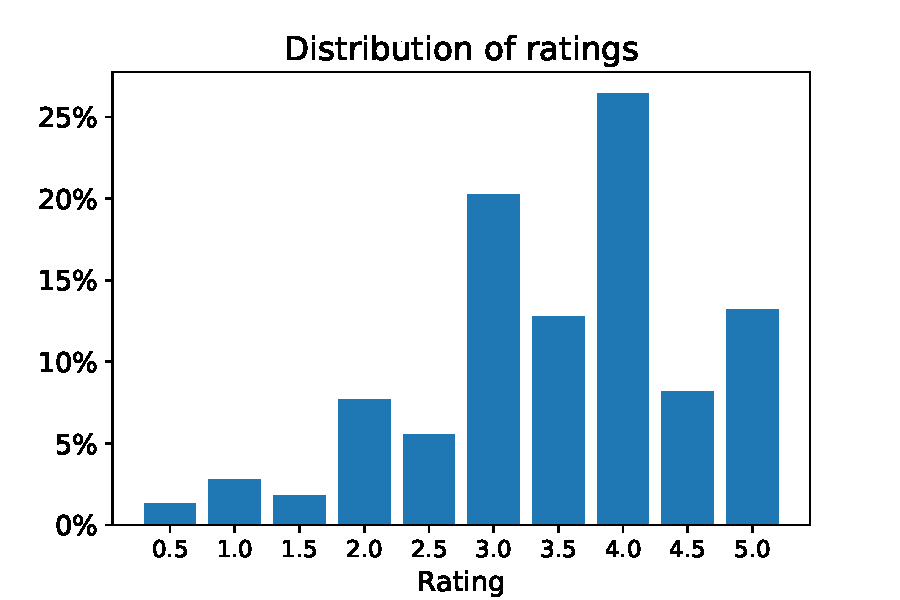
\includegraphics[width=1\linewidth]{img/ratings_dist.pdf}
    \end{figure}
    
  \end{frame}



  \begin{frame}
    \frametitle{Exploring the dataset cont'd}

    \begin{figure}
      \centering
      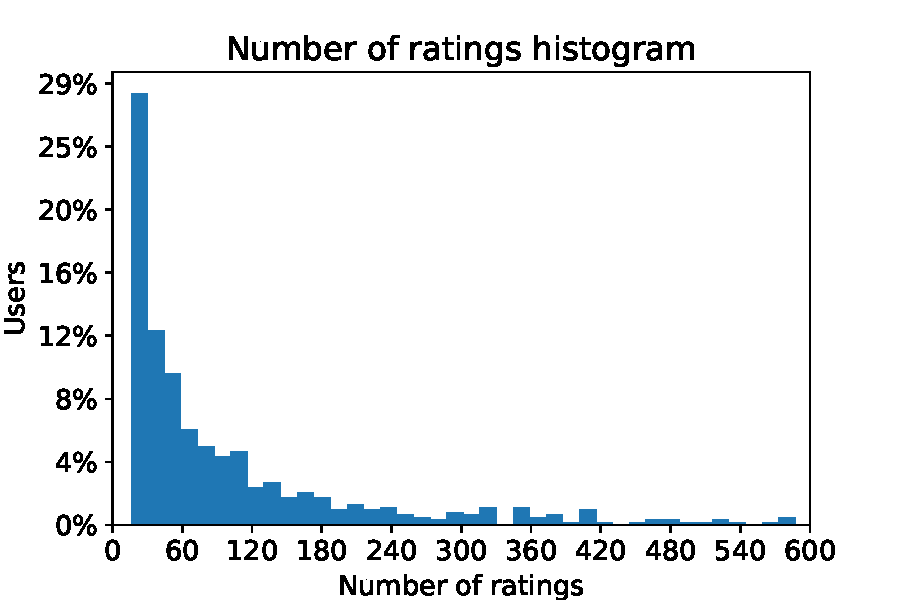
\includegraphics[width=0.9\linewidth]{img/n_ratings.pdf}
    \end{figure}

    Matrix sparsity: $1.59\%$. 

  \end{frame}



  \begin{frame}
    \frametitle{Mathematical setting}
    Formally, the model is based on matrix factorisation.
    \vspace{1em}
    \begin{itemize}
      \setlength\itemsep{1em}
    \item Aim: $ \underset{\scriptscriptstyle{M \times N}}{R} \approx \widetilde{R} = \underset{\scriptscriptstyle{M\times k}}{X}\underset{\scriptscriptstyle{k\times N}}{Y}$, with $k$ latent factors;
      \item Objective function:
        \begin{center}
          $\sum_{u, i} c_{ui} (r_{ui} - \mathbf{x_u^T y_i})^2 + \lambda \left( \sum_u \norm{\mathbf{x_u}}^2 + \sum_i \norm{\mathbf{y_i}}^2 \right)$;
        \end{center}
      \item Non-convex problem, solved using Weighted Alternating Least Squares;
      \item $\lambda$ determined using CV;
    \end{itemize}
  \end{frame}



  \begin{frame}
    \frametitle{Choice of weights}

    The choice of weights is problem dependent. Let $c_i = \sum_{u, i} 1$ if $r_{ui} > 0$.\\

    \vspace{1em}

    Explicit feedback:

    \begin{itemize}
      \setlength\itemsep{1em}
      \item $c_{ui} = \omega_0 + \omega_1 c_i$, where $\omega_0$ weights the unobserved entries, and $\omega_1$ the observed ones.
    \end{itemize}
    \vspace{1em}
    Implicit feedback:\\
    \begin{itemize}
      \setlength\itemsep{1em}
      \item $C = 1 + \alpha R$, where $\alpha =  40$ provides good results \cite{collaborative}.
    \end{itemize}

    \vspace{1em}

    Both choices lead to dense problems: this is preferable in order to avoid folding.

  \end{frame}



  \begin{frame}[fragile]\label{math}
    \frametitle{Performance concerns}

    Analytical solution for WALS:


    \begin{center}
      $\mathbf{x_u} = (Y^TC^uY + \lambda I)^{-1}Y^TC^u\mathbf{r_u}$
      \quad
      \hyperlink{math.aux}{\beamerbutton{AUX}}
    \end{center}

    Where $C^u = diag(\mathbf{c_u})$.\\
     
    \vspace{1em}

    For $n$ users and $k$ latent factors, the computation is $O(k^3 + k^2n)$ for each of the $m$ users.

    \vspace{1em}

    \pause

    \begin{lstlisting}
for u in range(1, M):
    Cu = diag(C[u,:])
    A = multi_dot([Y.T, Cu, Y]) + lam * eye(K)
    b = multi_dot([Y.T, Cu, R[u, :]])
    X_u = solve(A, b)
    \end{lstlisting}

    Note: this is embarrassingly parallel!

  \end{frame}



  \begin{frame}
    \frametitle{Cross validation}

    The best value for the regression coefficient $\lambda$ can be determined using cross validation.\\

    \vspace{1em}

    Splitting into train and test set for CV:

    \vspace{0.5em}

    \begin{itemize}
      \setlength\itemsep{0.5em}
      \item Cannot trivially split the rows of $R$;
      \item Random \texttt{(user, item)} pairs should be selected;
      \item If $C = 1 + \alpha R$, models with different values of $\alpha$ cannot be compared.
    \end{itemize}

    \vspace{1em}

    \pause

    Choice of error function:

    \vspace{0.5em}

    \begin{itemize}
      \setlength\itemsep{1em}
    \item $RMSE = \sqrt{\frac{1}{ |\widetilde{R}|} \sum_{u,i\in \widetilde{R}} (r_{ui} - \widetilde{r}_{ui})^2}$
    \item $MAE = \frac{1}{ |\widetilde{R}|} \sum_{u,i\in \widetilde{R}} \envert{r_{ui} - \widetilde{r}_{ui}}$
    \end{itemize}

  \end{frame}



  \begin{frame}
    \frametitle{Cross validation: results}

    \begin{figure}
      \centering
      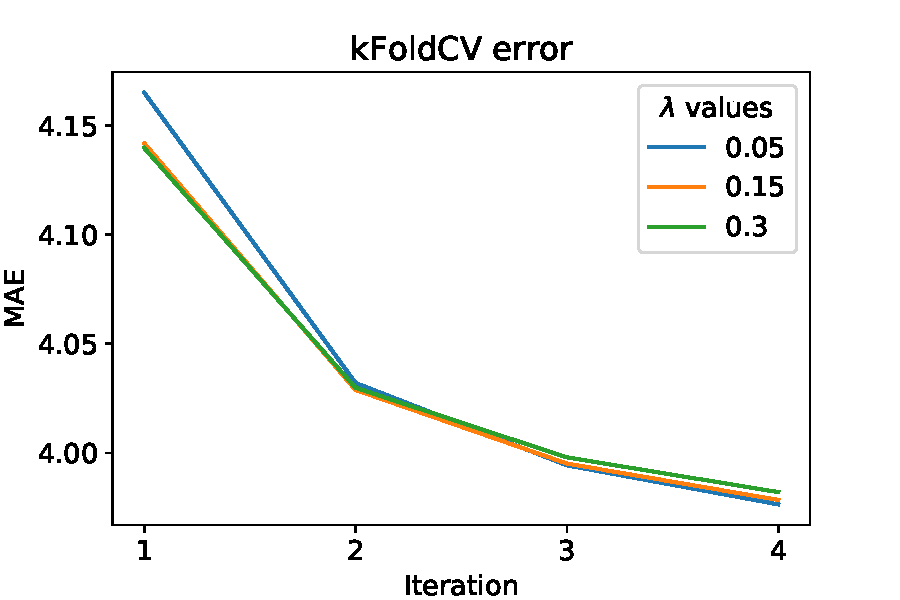
\includegraphics[width=0.9\linewidth]{img/TestErrorCV.pdf}
    \end{figure}

    Execution time: $\approx 3\, h$ for $4$ iterations and $k = 100$.\\What is the meaning of the high MAE?

  \end{frame}



  \begin{frame}
    \frametitle{Matrix factorisation}

    \begin{figure}
      \centering
      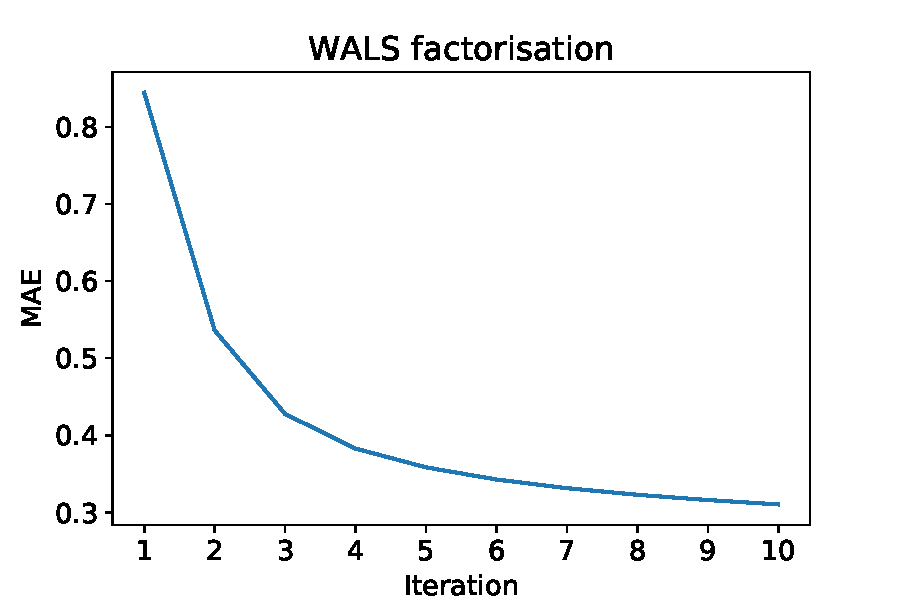
\includegraphics[width=.9\linewidth]{img/WALS_train.pdf}
    \end{figure}

    Execution time: $\approx 52\, min$ for $10$ iterations, $k = 100$ and $\lambda = 0.15$.

  \end{frame}



  \begin{frame}
    \frametitle{Recommendation results}

    \begin{center}
    \captionof*{table}{Recommended movies for \texttt{user\_id = 2}:}
    \scalebox{0.75}{
		\rowcolors{1}{}{ThemeRed!05}
      \begin{tabular}{rllr}
        \toprule
         Pred. & Title & Genres & AVG\_Rat. \\
        \midrule
        6.82 & Reservoir Dogs (1992) & Crime-Mystery-Thriller & 4.2 \\
        6.60 & Dances with Wolves (1990) & Adventure-Drama-Western & 3.8 \\
        5.89 & Gostbusters (1984) & Action-Comedy-Sci-Fi & 3.7 \\
        5.32 & American History X (1998) & Crime-Drama & 4.2 \\
        4.79 & Star Wars: Episode VI (1983) & Action-Adventure-Sci-Fi & 4.1 \\
        4.29 & Dave (1993) & Comedy-Romance & 3.5 \\
        4.24 & Fargo (1996) & Comedy-Crime-Drama-Thriller & 4.1 \\
        4.17 & Independence Day (1996) &  Action-Adventure-Sci-Fi-Thriller & 3.3 \\
        4.14 & Young Frankenstein (1974) & Comedy-Fantasy & 3.9 \\
        4.10 & Angels in the Outfield (1994) & Children-Comedy & 2.3 \\
        \bottomrule
      \end{tabular}
    }
    \end{center}


  \end{frame}



  \begin{frame}
    \frametitle{Recommendation results cont'd}

    \begin{center}
    \captionof*{table}{Best rated movies for \texttt{user\_id = 2}:}
    \scalebox{0.75}{
		\rowcolors{1}{}{ThemeRed!05}
      \begin{tabular}{llr}
        \toprule
         Title & Genres &  Rating \\
        \midrule
           Android (1982) & Sci-Fi & 5.0 \\
           Escape from L.A. (1996) & Action-Adventure-Sci-Fi-Thriller & 5.0 \\
           Saturn 3 (1980) & Adventure-Sci-Fi-Thriller & 5.0 \\
           The Lair of the White Worm (1988) & Comedy-Horror & 5.0 \\
           Road Warrior, The (Mad Max 2) (1981) & Action-Adventure-Sci-Fi-Thriller & 5.0 \\
           Hangar 18 (1980) & Action-Sci-Fi-Thriller & 5.0 \\
           Galaxy of Terror (Quest) (1981) & Action-Horror-Mystery-Sci-Fi & 5.0 \\
           Piranha (1978) & Horror-Sci-Fi & 4.5 \\
           Conan the Barbarian (1982) & Action-Adventure-Fantasy & 4.5 \\
           Looker (1981) & Drama-Horror-Sci-Fi-Thriller & 4.5 \\
        \bottomrule
      \end{tabular}
    }
    \end{center}


  \end{frame}



  \begin{frame}
    \frametitle{System evaluation}

    Recommender system can be evaluated using two approaches.

    \vspace{1em}

    Offline evaluation (easier to compare algorithms):
    \begin{itemize}
      \item Low test RMSE/MAE;
      \item High precision/recall;
      \item Decent catalogue coverage.
    \end{itemize}

    \vspace{0.5em}

    Online evaluation:
    \begin{itemize}
      \item A/B testing (measuring Click-Through Rate and Conversion Rate).
    \end{itemize}

    \vspace{1em}

    \pause

    My results for system evaluation:

    \begin{itemize}
      \item For each user, the 10 most recent ratings are used for testing;
      \item Mean precision and recall at 10: $2.8\%$.
    \end{itemize}

  \end{frame}


  
  \begin{frame}
    \frametitle{Similar items}

    Once the factorisation has been performed, the $Y$ matrix contains a representation of the items using $k$ latent factors.

    \vspace{1em}

    Using the item embedding we can, for a given movie, suggest the most similar movies in the dataset:

    \vspace{1em}

    \begin{itemize}
      \setlength\itemsep{1em}
    \item For a given \texttt{movie\_id} $i$, compute the cosine similarity with all the other movies $j$ as

        \begin{center}
          $\text{sim}(i, j) = \displaystyle\frac{\mathbf{y}_i \cdot \mathbf{y}_j}{\norm{\mathbf{y}_i} \cdot \norm{\mathbf{y}_j}}$
        \end{center}

      \item Return a ranked list, sorting the resulting movies by their similarity.
    \end{itemize}

    \vspace{1em}

    Note, the similarity is $\in [-1, 1]$

  \end{frame}



  \begin{frame}
    \frametitle{Similar items: results}

    \begin{center}
    \captionof*{table}{Similar to: "The Lord of the Rings: The Fellowship of the Ring"}
    \scalebox{0.75}{
		\rowcolors{1}{}{ThemeRed!05}
      \begin{tabularx}{1.3\textwidth}{lXr}
        \toprule
        Title & Genres & Similarity \\
        \midrule
        LOTR: The Fellowship of the Ring & Adventure-Fantasy & 1.00 \\
        LOTR: The Return of the King & Action-Adventure-Drama-Fantasy & 0.83 \\
        LOTR: The Two Towers & Adventure-Fantasy & 0.79 \\
        The Sixth Sense & Drama-Horror-Mystery & 0.78 \\
        In the Name of the Father & Drama & 0.77 \\
        Twelve Monkeys & Mystery-Sci-Fi-Thriller & 0.79 \\
        \bottomrule
      \end{tabularx}
    }
    \end{center}

    \begin{center}
    \captionof*{table}{Similar to: "Star Wars: Episode VI - The Return of the Jedi"}
    \scalebox{0.75}{
		\rowcolors{1}{}{ThemeRed!05}
      \begin{tabularx}{1.3\textwidth}{lXr}
        \toprule
        Title & Genres & Similarity \\
        \midrule
        Star Wars: Episode VI & Action-Adventure-Sci-Fi & 1.00 \\
        Star Wars: Episode V & Action-Adventure-Sci-Fi & 0.69 \\
        The Silence of the Lambs & Crime-Horror-Thriller & 0.61 \\
        Independence Day & Action-Adventure-Sci-Fi-Thriller & 0.58 \\
        Star Wars: Episode IV & Action-Adventure-Sci-Fi & 0.55 \\
        Gladiator & Action-Adventure-Drama & 0.54 \\
        \bottomrule
      \end{tabularx}
    }
    \end{center}

  \end{frame}



  \begin{frame}
    \frametitle{Recommendation for new users}

    What if a new user (a set of rated movies on which the system has not been trained) asks for recommendations?

    \vspace{1em}

    \begin{itemize}
      \item Naive solution: add the new user to the $R$ matrix and recompute the factorisation.
    \end{itemize}

    \vspace{1em}

    This is slow and computationally demanding.

    \vspace{1em}

    \begin{itemize}
      \item Better/faster solution: keep the item embedding $Y$ fixed and compute a single iteration of the WALS algorithm.
    \end{itemize}

    \vspace{1em}

    But we need to assume that $Y$ does not change much if a few users are added into the system. If it does change, a full factorisation should be performed. 

  \end{frame}



  \begin{frame}[fragile]
    \frametitle{Recommendation for new users cont'd}

    For a new user $M + 1$:

    \vspace{0.5em}

    \begin{enumerate}
      \setlength\itemsep{0.5em}
      \item Take $Y$ from full matrix factorisation;
      \item Obtain a user representation $\mathbf{x}_{M+1}$ (a single linear system!);
      \item Compute the predicted ratings $\mathbf{r}_{M+1} = \mathbf{x}_{M+1}Y$ and sort items by their score.
    \end{enumerate}

    \vspace{1em}

    \begin{lstlisting}
u = M + 1
Cu = diag(C[u,:])
A = multi_dot([Y.T, Cu, Y]) + lam * eye(K)
b = multi_dot([Y.T, Cu, R[u, :]])
X_u = solve(A, b)
    \end{lstlisting}

  \end{frame}



  \begin{frame}
    \frametitle{New users: results}

    New user with $50$ randomly rated movies.

    \begin{center}
    \captionof*{table}{Recommended movies:}
    \scalebox{0.75}{
		\rowcolors{1}{}{ThemeRed!05}
      \begin{tabularx}{1.3\textwidth}{lllX}
        \toprule
        Prediction & Title & Genres & AVG\_Rating \\
        \midrule
        7.70 & Apocalypse Now & Action-Drama-War & 4.2 \\
        6.76 & Zodiac & Crime-Drama-Thriller & 3.7 \\
        6.31 & Singin' in the Rain & Comedy-Musical-Romance & 4.1 \\
        6.03 & ToCatcha Thief & Crime-Mystery-Romance-Thriller & 4.2  \\
        5.87 & Malcolm X & Drama & 4.1\\
        \bottomrule
      \end{tabularx}
    }
    \end{center}

    \begin{center}
    \captionof*{table}{Best rated movies:}
    \scalebox{0.75}{
		\rowcolors{1}{}{ThemeRed!05}
      \begin{tabularx}{1.3\textwidth}{llX}
        \toprule
        Title & Genres & Rating \\
        \midrule
        Once Upon a Time in China & Action-Adventure-Drama & 5.0 \\
        Picnic at Hanging Rock & Drama-Mystery & 5.0 \\
        Kung Fu Panda: Secrets of the Masters & Animation-Children & 5.0\\
        $\text{[REC]}^2$ & Horror-Thriller & 5.0\\
        In the Heat of the Night & Drama-Mystery & 5.0\\
        \bottomrule
      \end{tabularx}
    }
    \end{center}

  \end{frame}



  \begin{frame}
    \frametitle{Cold start problem: users}

    What if a new user has rated too few movies or even no movie at all?

    \vspace{1em}

    If possible, gather information:

    \vspace{0.5em}

    \begin{itemize}
      \item Old MovieLens approach: new users must rate 15 movies;
      \item New MovieLens approach: choose among groups of related movies;
      \item Use cross-domain information (i.e., book ratings);
      \item If personality/social network information is available, link similar users;
    \end{itemize}

    \vspace{0.5em}

    If no feedback and no information are available, provide popularity-based or random recommendations.

  \end{frame}



  \begin{frame}[fragile]
    \frametitle{Cold start problem: users cont'd}

    Proposed solution:

    \vspace{1em}

    \begin{lstlisting}[
    basicstyle=\footnotesize,
]
Too few movies! Most poular movies will be suggested.
    \end{lstlisting}

    \begin{center}
    \scalebox{0.75}{
		\rowcolors{1}{}{ThemeRed!05}
      \begin{tabularx}{1.3\textwidth}{Xlrr}
        \toprule
        Title & Genres & AVG\_Rat & Counts \\
        \midrule
        Forrest Gump & Comedy-Drama-Romance-War & 4.1 & 322 \\
        Shawshank Redemption, The & Crime-Drama & 4.4 & 315 \\
        Pulp Fiction & Comedy-Crime-Drama-Thriller & 4.1 & 307 \\
        Matrix, The & Action-Sci-Fi-Thriller & 4.1 & 263 \\
        Star Wars: Episode IV& Action-Adventure-Sci-Fi & 4.2 & 251 \\
        Braveheart & Action-Drama-War & 4.0 & 237 \\
        Silence of the Lambs, The & Crime-Horror-Thriller & 4.1 & 232 \\
        Jurassic Park & Action-Adventure-Sci-Fi-Thriller & 3.7 & 219 \\
        \bottomrule
      \end{tabularx}
    }
    \end{center}

    \vspace{1em}

    In real cases, take care of \textit{popularity bias}.

  \end{frame}



  \begin{frame}[fragile]
    \frametitle{Cold start problem: movies}

    What if a movie in the dataset has few/no ratings? 

    \vspace{1em}

    This is not a problem for content-based filtering, which needs no historical information about items.

    \vspace{1em}

    For collaborative filtering:

    \vspace{0.5em}

    \begin{itemize}
      \item Ask users for help (e.g., ExcUseMe algorithm \cite{useme});
      \item Use a freshness measure.
    \end{itemize}

    \vspace{0.5em}

    \pause

    A concrete instance: computing cosine similarity with null rows in item embedding (caused by too few/no interactions for the item).

    \vspace{0.5em}

    \begin{lstlisting}[basicstyle=\footnotesize]
# Computing sim(y_i, y_j).
if len(y_i) == 0 or len(y_j) == 0:
    return -1
    \end{lstlisting}



  \end{frame}



  \begin{frame}
    \frametitle{Possible improvements and Conclusions}

    How could the current system be improved?

    \vspace{0.5em}

    \begin{itemize}
      \setlength\itemsep{0.5em}
      \item Use a larger dataset;
      \item Parallelise matrix factorisation;
      \item Implement a freshness measure;
      \item Include a static score (rating) or freshness score in computing similarity;
      \item Include a diversity measure (aiming at serendipity).
    \end{itemize}

    \vspace{2em}

    \begin{block}{Conclusions}
      Despite the poor quantitative evaluations, the system seems to perform decently both with recommendation of new movies and of similar movies.
    \end{block}

  \end{frame}



  \begin{frame}
    \frametitle{References}

    \nocite{*}

    \setbeamercolor{bibliography entry author}{fg=ThemeRed}
    \setbeamercolor{bibliography entry title}{fg=black} 
    \setbeamercolor{bibliography entry location}{fg=black} 
    \setbeamercolor{bibliography entry note}{fg=black}  
    \setbeamercolor{bibliography item}{fg=ThemeBlue}
    \setbeamertemplate{bibliography item}[text]

    \bibliographystyle{abbrv}
    \footnotesize{
      \bibliography{biblio.bib} 
    }
  \end{frame}

  

  % Auxiliary slides.
  \appendix
  % Beginning of backup slides, do not count pages.
  \backupbegin

  \section{Auxiliary slides}


  \begin{frame}\label{math.aux}
    \frametitle{WALS: analytic solution}

    Starting from the objective function

    \begin{center}
      $\mathcal{L} = \sum_{u, i} c_{ui} (r_{ui} - \mathbf{x_u^T y_i})^2 + \lambda \left( \sum_u \norm{\mathbf{x_u}}^2 + \sum_i \norm{\mathbf{y_i}}^2 \right)$:
    \end{center}

    \vspace{1em}

    \begin{itemize}
      \setlength\itemsep{1em}
      \item $\frac{\partial \mathcal{L}}{\partial \mathbf{x_u}} = -2\sum_i c_{ui}(r_{ui} - \mathbf{x_u^T y_i}) \mathbf{y_i} + 2\lambda \mathbf{x_u} = 0$
      \item Scalar product commutativity:
        \vspace{0.3em}
        \begin{center}
          $-2\sum_i c_{ui}(r_{ui} - \mathbf{y_i^T x_u}) \mathbf{y_i} + 2\lambda \mathbf{x_u} = 0$
        \end{center}
      \item Using the definition of matrix product:
        \vspace{0.3em}
        \begin{center}
          $-2Y^TC^u\mathbf{r_u}+2Y^TC^uY\mathbf{x_u}+2\lambda \mathbf{x_u} = 0$
        \end{center}
      \item Rearranging:
        \vspace{0.3em}
        \begin{center}
          $\mathbf{x_u} = (Y^TC^uY + \lambda I)^{-1}Y^TC^u\mathbf{r_u}$
        \end{center}
    \end{itemize}

  \end{frame}


  \backupend



\end{document}
